\documentclass[11pt]{article}
\usepackage{cite}
\usepackage{lmodern}
\usepackage[utf8]{inputenc}
\usepackage[finnish]{babel}
\usepackage{hyperref}
\usepackage{graphicx}
\usepackage[figurename=Fig.]{caption}
\usepackage{subfig}


\title{Network Analysis - Project Report}
\author{
    Jimi Hytönen\\
    \and Hanna Holtdirk\\
    \and Basil Mashal
}
\begin{document}

\maketitle

\section{Introduction}
This project is part of network analysis course. The purpose of this project was to analyse real-world network by applying different algorithms to extract some interesting information about the network as well as get hands-on experience with network analysis. We chose to analyse California road networks because TBD - why? 


In this report we will cover the technical aspects of gathering the data, tell how the work was divided, explain our network analysis and visualizations, and finally describe our conclusions. The project can be found in github (https://github.com/Jimmeeee/NA-project)



\section{Data}

We used dataset from https://www.cs.utah.edu/~lifeifei/SpatialDataset.html which was collected, cleaned and formated from multiple different sources into easy-to-use format. Network's nodes were in longitude-latitude coordinate form and network's edges contained information about start node, end node and the distance between them. In addition, the site provided information about California's points of interests such as hospitals, lakes and airports.

We used pandas for data manipulation and processing as we needed to get the data into a certain form for further analysis. We used networkx for building and visualisation of the network. This was really straightforward to do as the data was in an easy to use format.  TBD-something else?

\newpage

\section{Methods}
For the project we divided the original question into the following subtasks: 
\begin{enumerate}
\item What is the general structure of the road network
\item Can we find where the (big) cities are from the road network and points of interest
\item Can we learn to make predictions about the placement of the roads and places of interest
\end{enumerate}

For each of these subtasks we planned what analysis was needed to answer the question. After setting these subtasks we created a timeline for the project. 

For the first question we analysed the California road network with simple methods to get a better idea what we are dealing with. One of which was calculating the connectivity of the network to determine if there were roads that led nowhere. We also calculated and visualized different centrality measures of the network such as degree centrality, betweenness centrality, eigenvector centrality and katz centrality. 

After analysing the general structure of the network, we moved to the second question. For finding the big cities we used Girvan Newman community detection algorithm as it seemed to be the most suitable for the task. However, we didn't use the algorithm on the whole network because it was enormous, instead we used approximation based on previously calculated centrality measures to create a smaller graph and applied the algorithm on that.

For the third question ...

\newpage

\section{Results}
\subsection{General structure analysis results}

\subsubsection{Visualisation}
We visualised the network using python library called networkx. In the following figure we can see the edge structure of California's road network on the left, and on the right we can see the same graph but with intensity of edge based on number of points of interest.
\begin{figure}[h!]
    \centering
    \caption{California's road network}%
    \subfloat[Edges on the network]{{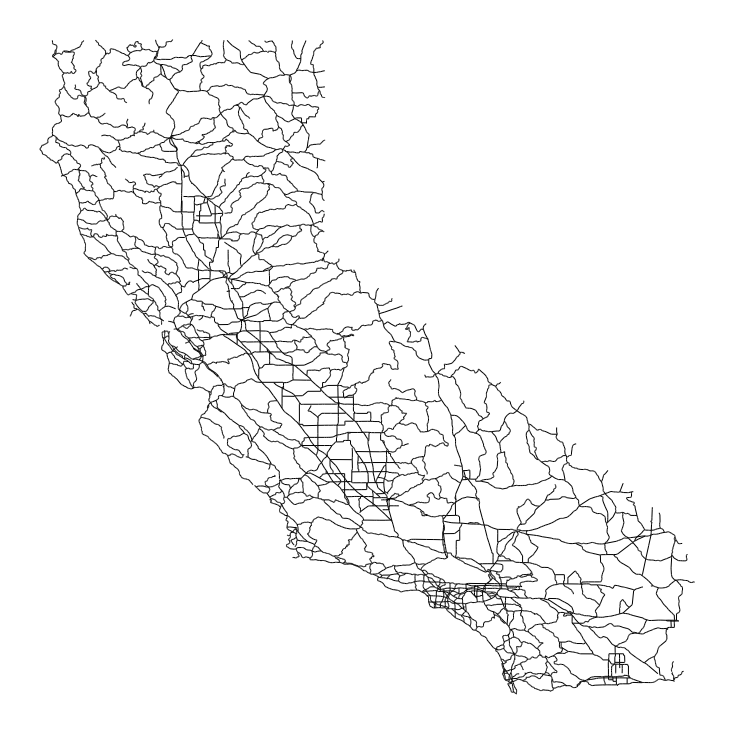
\includegraphics[width=5.5cm]{road.png} }}%
    \qquad
    \subfloat[Points of interest edge intensity]{{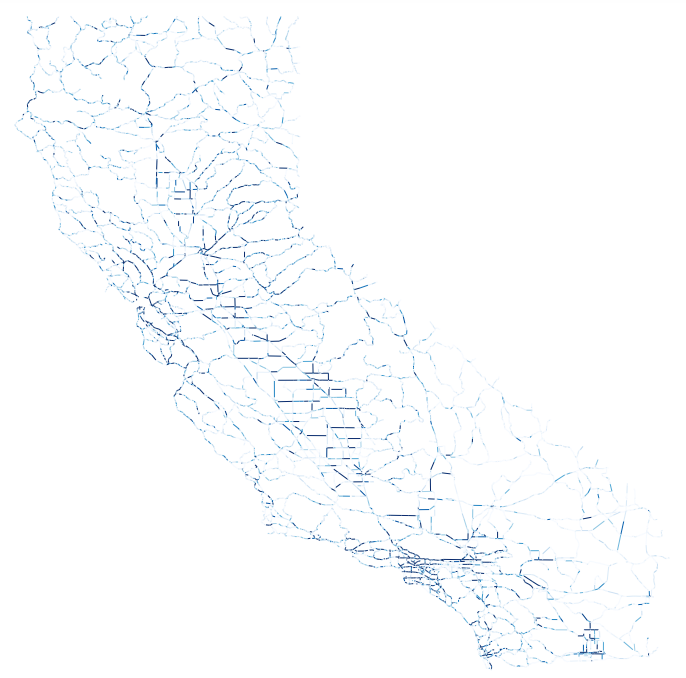
\includegraphics[width=5.5cm]{merge.png} }}%
\end{figure}




\subsubsection{Degree distribution}
In order to get more information about the basic structure of the network we checked the connectivity of the network and analysed degree distribution of the nodes. We found out that the California's roads are connected and there are no isolated sections. Also, from the figure below we can see the node degree distributions. It is intuitive that the majority of the nodes have degree of two as they are the middle nodes of the road. However, we can also see that there are lots of nodes that have degree higher than two, they are the intersections. Nodes that have degree of one are dead-ends.

\begin{figure}[h]
\caption{Degree distribution}
\centering
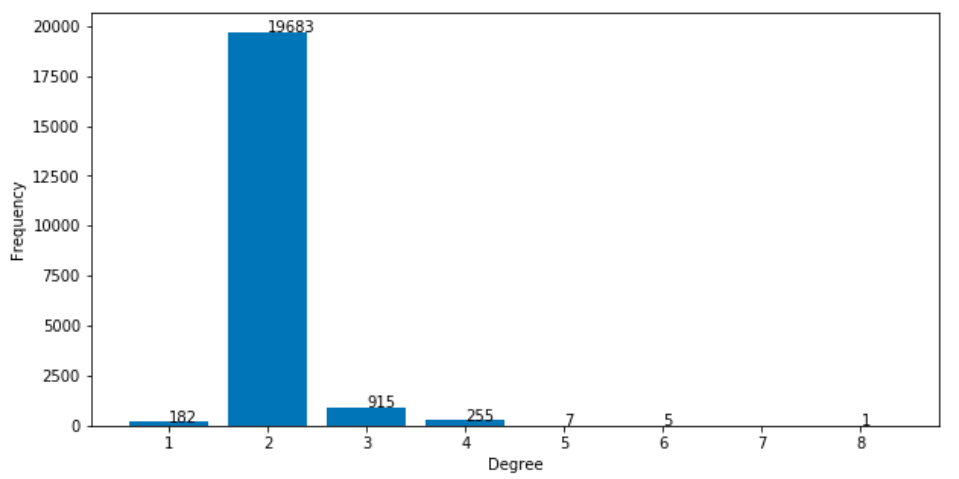
\includegraphics[scale=0.4]{degree.png}
\end{figure}

\subsubsection{Centrality}
We analysed the structure of the network with different centrality measures. These were: degree centrality, betweenness centrality, eigenvector centrality and katz centrality. In the figure below we can see the different centrality measures where higher color intensity and bigger node size means higer centrality value.  

\begin{figure}[h!]
\centering
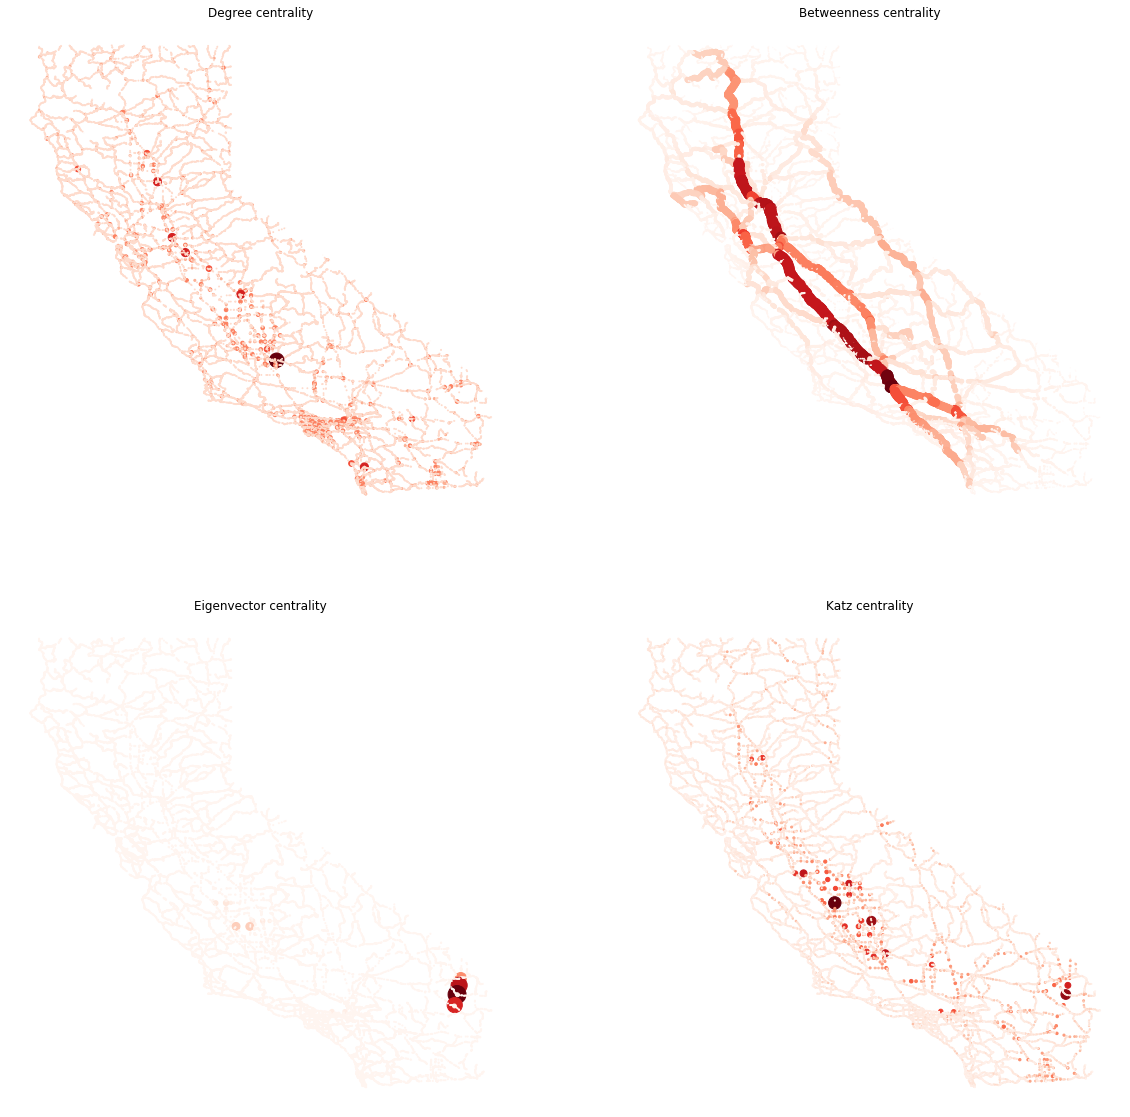
\includegraphics[scale=0.24]{centrality.png}
\end{figure}


\subsection{Communitites}
For finding out the counties of California we used Girvan Newman community detection algorithm on networkx. Since the size of our network was inormous we had to optimize the algorithm with few methods. We based our edge removal to betweenness centrality as it sped up the algorithm noticeably. Also, we stopped the algorithm after it had found 58 communities as there are only 58 counties in California. In the figure below we can see how well we managed to find different counties based on the road network. 

\begin{figure}[h!]
\title{Girvan Newman community detection}
\centering
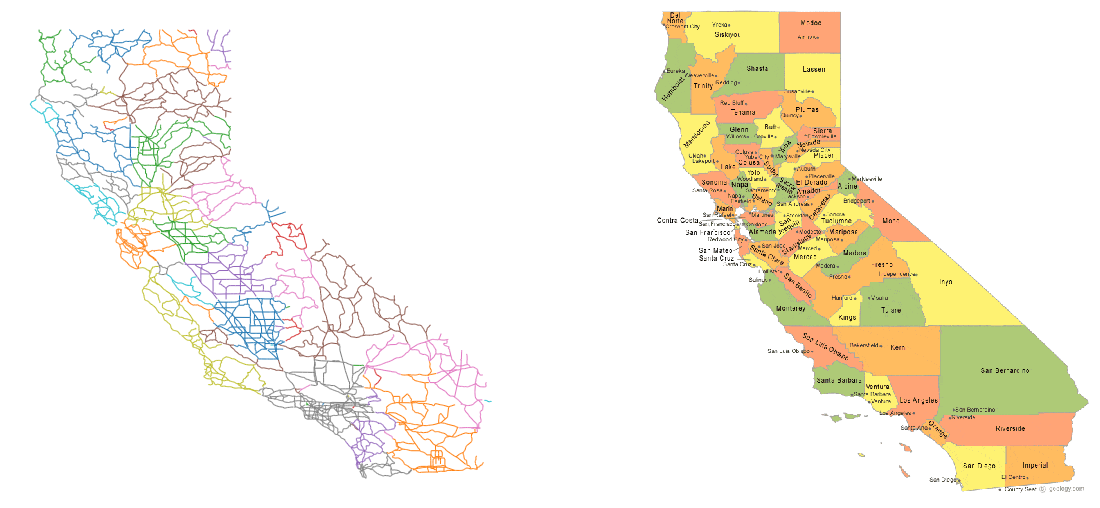
\includegraphics[scale=0.4]{community.png}
\end{figure}

\subsection{Machine Learning}


\newpage
\section{Conclusions}
This does not need to be long


\section{Contributors}

\begin{enumerate}
    \item Jimi Hytönen - Gathering data, building and visualising the network. Helping out with general structure and communities. Writing project report.
	\item Hanna Holtdirk - TBD
	\item Basil Mashal - TBD

\end{enumerate}


\end{document}
